\documentclass{article}
\usepackage{graphicx} % this package can be used for inserting graphics
\usepackage{amsmath} % this package includes the align environment
%\usepackage{minted} % while not correctly configured at present, the minted package can be used
% to display code snippets with syntax highlighting in your documents. Notepad++
% can also print PDFs of syntax highlighted code.
\begin{document}
\title{CS3505 Final Project, Fall 2020} %Don't forget to change the title.
\author{Team Exoplanets\\Edward Barrowes, Corbin Gurnee, Ted Goodell,\\Marley Stark, Ivan Burkett, Garrett Keefe}
% The (build) date is included by default
\maketitle
\newpage

\section{Overview}
  % Use prose to briefly describe your project and intended features
\section{Architecture}
  \subsection{Organization}
  % Use prose and UML as appropriate to describe how your project parts are organized.

  % AWS runs a virtual machine (EC2), which runs continuously and runs docker images at regular time intervals using cron
  % EC2 runs docker containers using Dockerfiles we have made
  % 1 image has 6 containers which use python to collect data from their individual sources
  % Data is stored in the EFS (elastic file storage) in the form of images
  % At a time specified by the user, a video is built (framebuilder.cpp does this)
  %  framebuilder.cpp, which exists in the EFS, is run by the user.
  %   framebuilder.cpp calls ffmpeg code to make 600 frames, stored in EFS
  % The user runs an ffmpeg command to put the frames together, which outputs a video to whatever directory you want
  %   this happens in the same place that framebuilder exists (EFS)

  \begin{figure}[h!]
    \includegraphics{uml_class_diagram.png}
    \caption{text}
    \label{}
  \end{figure}

  \subsection{Execution}
  % Use prose and UML as appropriate to describe how your project parts execute.
  \begin{figure}[h!]
    \includegraphics{uml_lifeline.png}
    \caption{}
    \label{}
  \end{figure}

  \subsection{Version Control}
  % Describe the architecture and revision control of your source code.
  % You should not reinvent all this now – just put in your report your design documents / design UML, polished and made readable / professional.

\section{Development}
  \subsection{Organizational Tools}
  % Write a brief summary of the tools used to organize your project.
  % Write/provide documentation from your planning software
  \begin{figure}[h!]
    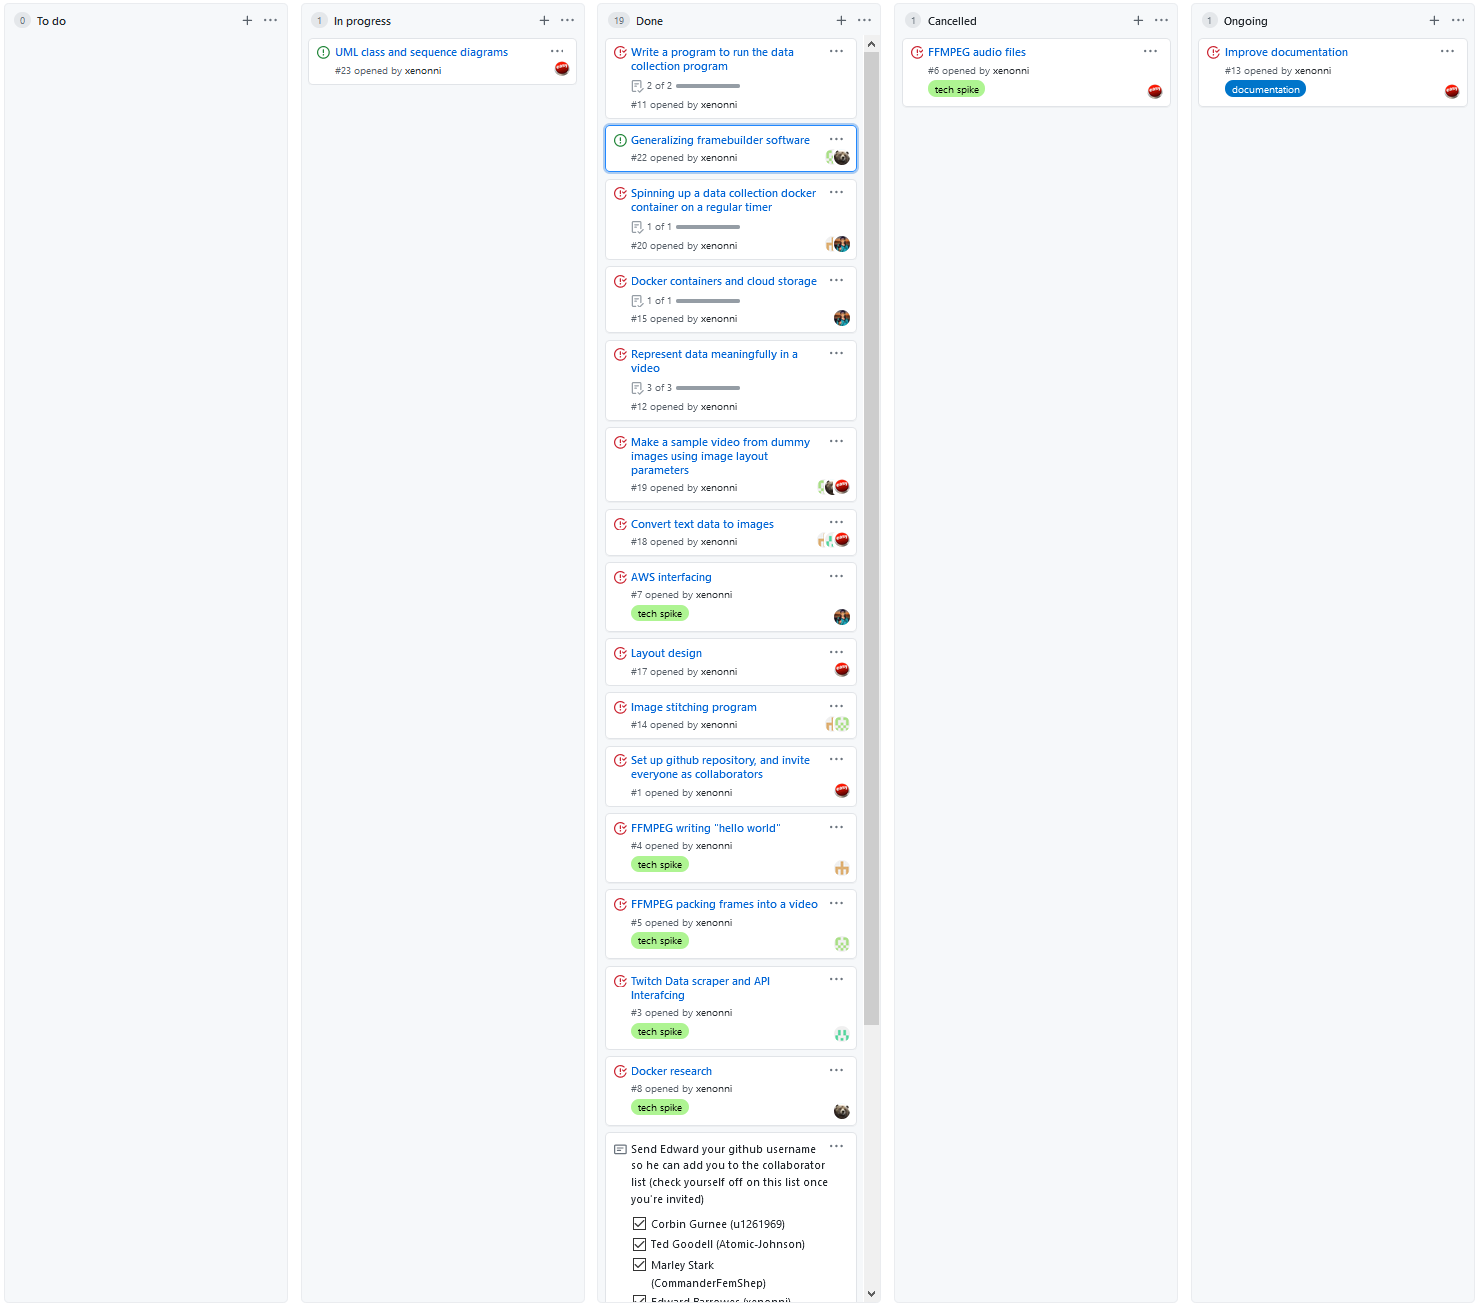
\includegraphics{github_projects.png}
    \caption{}
    \label{}
  \end{figure}

  \begin{figure}[h!]
    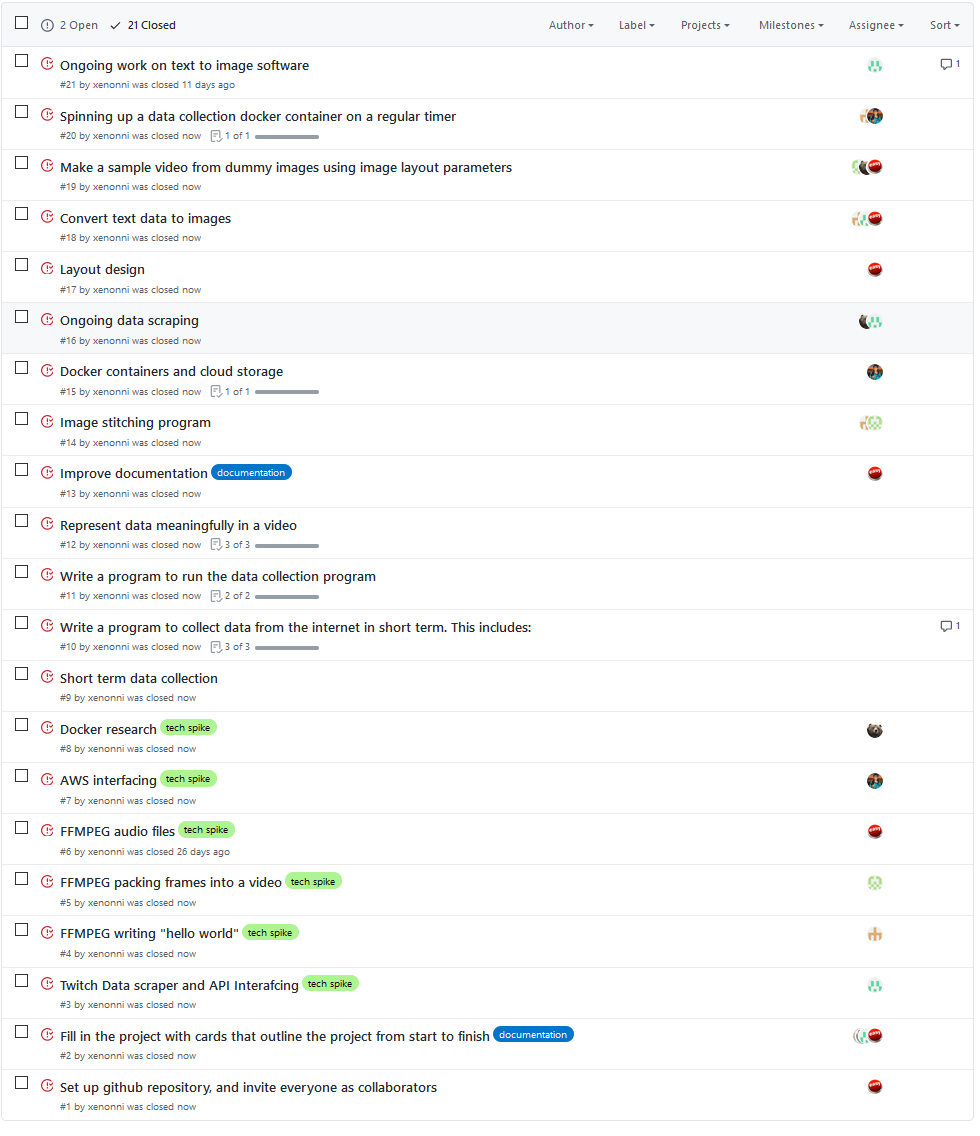
\includegraphics{task_backlog.png}
    \caption{}
    \label{}
  \end{figure}
  % Attach all the meeting notes as an appendix
  \subsection{Individual Reports}
    \paragraph{Corbin Gurnee -}
    For this project, I assisted with multiple parts. I was assigned to figure out how to work with API’s and how to get data with them. Thus I created a script to use the API on Twitch to gather the number of people watching the Science and Technology channel. After this I worked with Garret to create a Web scraper to get images off a webpage online. This turned out to be much easier than interacting with an API, so we changed all other scripts to run off of the web scraper as well. After this, I worked with Ted to convert the data we have compiled from our web scrapers to images. Finally, I worked in limited capacities with most other members of the team to assist in any area they may need assistance with.
    \paragraph{Ted Goodell -}
    I worked with Ivan on using the ffmpeg libraries to combine multiple images into a single image. To do this, we wrote code that decoded several images from their files and put them into frame structs that we could then programmatically combine into a larger frame. We then used the ffmpeg libraries to encode that frame and put it into an output image. I also, wrote python scripts that grabbed text data output by the data grabbers, and used the ffmpeg command line utility to put that text into an image. The ffmpeg command used a built in filter called “drawtext” to draw the text on a black template image for that portion of the final output image.
    \paragraph{Ivan Burkett -}
    I was assigned to work on the frame builder program for this project. I worked with Ted to create a C++ program called image-smoosh.cpp that used ffmpeg to combine the 6 frame segments into a single frame, then saved that frame as a png image. After finishing image-smoosh.cpp, I refactored the program to make it cleaner and easier to read and saved it as image-smoosh2.cpp. After doing that, I used image-smoosh2.cpp as a base to create framebuilder.cpp with Garrett. As part of making framebuilder.cpp, I also created a wrapper class for the C++ class directory-iterator called peek-directory-iterator, which simplified usage for directory-iterator and added a peek functionality which was necessary for our file traversal algorithm. framebuilder.cpp uses peek-directory-iterators to scan through the data source folders for the one most up to date for the provided date during the frame building process.
    \paragraph{Garrett Keefe -}
    I first worked on gathering research on docker and how it works. Then I was assigned with Corbin to work on the data scrappers to collect data from our 6 sources. I wrote all of the .py files which used selenium to navigate and grab web resources while Corbin wrote the twitch.out file which uses C++ and the curl libraries to query twitch.tv for info from its API. After that I was assigned to working with Ivan to create the framebuilder program which utilize UNIX timestamps to assemble data from our data sources and compile them together into individual frames, allowing us to generate a list of frames which we use an ffmpeg command to assemble them into a video. I also helped Ted create all of the .sh files which acted as drivers for our data collection and converting to picture formats within the docker containers.
\section{Results}
  % Write prose to describe the current project functionality
  \subsection{Running the Code}
  % Briefly indicate requirements and steps for running the project code.
  \begin{figure}[h!]
    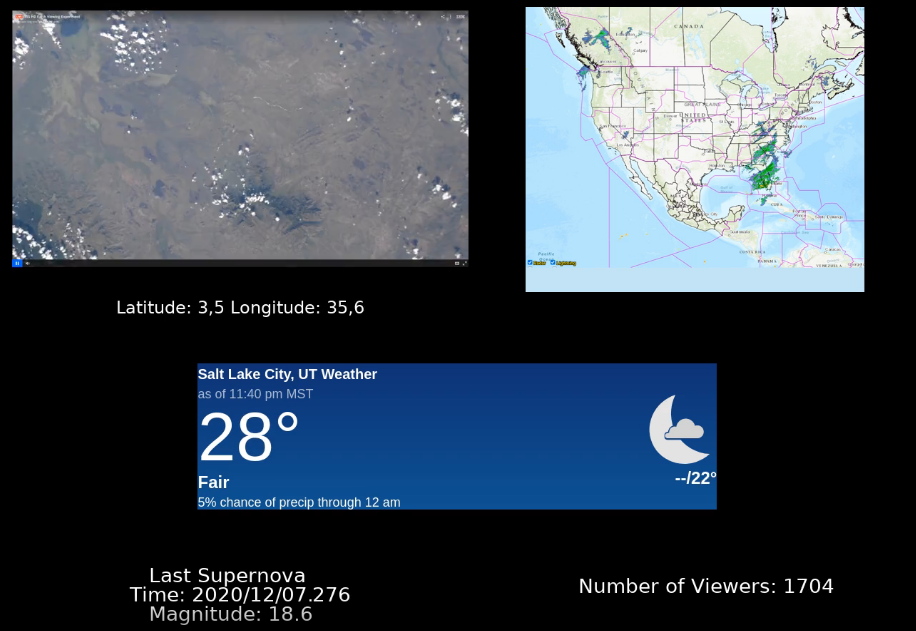
\includegraphics{timeline_screenshot.png}
    \caption{}
    \label{}
  \end{figure}

\section{Appendix A: Meeting Minutes}


\end{document}
